\chapter{Evaluation of the Adaptive Fusion Framework}


\section{7.1 Introduction}


This chapter evaluates whether the proposed framework achieved the research objectives defined in Chapter 1 and operationalized through the approach in Chapter 4. The evaluation focuses on classification performance, adaptive fusion behaviour, reliability feature contribution, robustness, and explainability. The results are reported cautiously because the final dataset is derived from one benchmark source and the multi-seed evaluation showed variation in reinforcement learning performance.


\section{7.2 Evaluation Strategy}


The evaluation was designed around five questions. First, the unimodal image and text branches were evaluated separately to determine the strength of each modality. Second, deterministic fusion baselines were compared with the proposed reinforcement learning fusion model. Third, ablation experiments tested whether reliability-aware state features improved the fusion controller. Fourth, policy and robustness analyses examined whether the model changed modality weights in meaningful ways. Fifth, explainability outputs were inspected to verify that image, text, and fusion-level explanations were generated.


The final evaluation evidence-flow diagram in this chapter makes these tests explicit. It is included to avoid presenting the final macro F1 score in isolation and to show how each examiner-facing question is connected to an artifact-backed test.


\section{7.3 Experimental Setup}


The implementation used Python, PyTorch, Transformers, pandas, scikit-learn, and image-processing libraries. Experiments were executed using Google Colab GPU runtime and Google Drive storage. The image branch used a pretrained ResNet-based model, and the text branch used a DistilBERT-based model. The fusion layer operated on low-dimensional reliability features rather than raw image or text embeddings, which kept the adaptive controller lightweight compared with the unimodal encoders.


\section{7.4 Dataset and Splits}


The experiments used the Fakeddit multimodal dataset. The full prepared metadata contained 682,661 rows after label standardization. For the final computable experiment, 28,000 balanced image-text samples were requested. Due to unavailable or failed image downloads, 26,471 samples were available for final multimodal evaluation. The final available splits contained 18,893 training rows, 3,798 validation rows, and 3,780 test rows.


The original Fakeddit two-way label was converted into the project label standard, where 0 represents real content and 1 represents fake content. Samples without available images were excluded from the final multimodal subset rather than being synthetically filled.


\section{7.5 Evaluation Metrics}


The main classification metrics were macro F1, accuracy, balanced accuracy, precision, recall, confusion matrix, and ROC-AUC. Macro F1 was treated as the primary metric because the task involves two classes and the evaluation should not rely only on overall accuracy. ROC-AUC was used to evaluate ranking quality from predicted probabilities. For policy analysis, average image weight, average text weight, action distribution, and group-wise metrics were also reported.


\section{7.6 Unimodal Branch Results}


The image-only branch achieved a test macro F1 of 0.7769 and test accuracy of 0.7791. The text-only branch achieved a test macro F1 of 0.8388 and test accuracy of 0.8389. These results show that the text branch was stronger than the image branch on the final test split. However, the image branch still contributed useful information because fusion methods improved over the text-only baseline.


The text branch also showed a visible overfitting gap: the training macro F1 was approximately 0.9882, while the test macro F1 was 0.8388. The model checkpoint was selected using validation performance, so the reported test result remains a held-out evaluation, but the gap indicates that stronger regularization or validation-loss-based selection should be considered in future work.


\section{7.7 Baseline and Fusion Results}


The final method comparison is summarized in Table 7.1 and visualized through the performance dashboard, confusion-matrix panel, and macro-F1 comparison figure. Image-only and text-only baselines were weaker than multimodal fusion. Equal fusion and confidence-weighted fusion both achieved test macro F1 of 0.8673. The proposed RL adaptive fusion model achieved test macro F1 of 0.8676 in the main final run. With validation-selected threshold tuning, RL adaptive fusion achieved test macro F1 of 0.8685.


The improvement over the strongest fixed fusion baseline was modest. Therefore, the result should be interpreted as competitive performance with a small main-run improvement, rather than as a large statistical superiority claim. The additional contribution of the proposed method is that it provides sample-level fusion actions and modality weights, which fixed fusion baselines do not provide.


The matched supervised MLP fusion baseline reached 0.8547 macro F1 at the default threshold and 0.8565 macro F1 after threshold tuning. This fairer comparison used the matched supervised fusion evidence files and shows that the adaptive RL fusion result remained stronger in the final reported run.

A paired McNemar audit aligned predictions by sample identifier before testing. The RL adaptive fusion run was not significantly different from equal fusion or confidence-weighted fusion at the default threshold (both p=1.0000). Against the matched supervised MLP fusion controller, however, the RL controller produced significantly more correct discordant decisions (b=95, c=46, p=0.000045). This supports the claim that the learned RL controller improved over the matched supervised controller, while fixed-fusion superiority remains a cautious and non-significant claim.


\section{7.8 Ablation Study}


The ablation study tested three reinforcement learning state representations and compared them with simple same-state controller baselines. The probabilities-only state achieved test macro F1 of 0.8523. Adding prediction confidence improved the score to 0.8590. The full reliability state, which included probability, confidence, quality, disagreement, confidence difference, and quality difference, achieved 0.8673. This pattern indicates that the reliability-aware features contributed meaningfully to the fusion controller.


\section{7.9 Policy Analysis and Reliability Behaviour}


The final policy analysis, including the weight-behaviour and action-distribution diagrams, showed that the RL fusion model used an average image weight of 0.6594 and an average text weight of 0.3406 on the test split. This indicates that the policy often assigned a larger contribution to the image branch in the selected final run. However, the action distribution also showed that the model did not use only one fixed weighting pattern.


When image and text branch predictions agreed, macro F1 was 0.9110. When they disagreed, macro F1 decreased to 0.7156, and the weights became more balanced, with average image weight 0.4987 and average text weight 0.5013. This behaviour is important because disagreement samples are harder and require more careful fusion decisions.


\section{7.10 Robustness Analysis}


Robustness tests were used to examine whether the fusion policy changed modality weights when modality quality or probabilities were corrupted. Under image quality degradation, the model reduced image weight as the degradation level increased, as shown in Figure 7.4. At degradation levels 0.25, 0.50, and 0.75, the image-weight changes were -0.0164, -0.0632, and -0.1283, respectively. Macro F1 decreased only slightly from 0.8671 to 0.8658 across these image-quality degradation levels.


The text-quality degradation behaviour was less consistent. In the tested configuration, the model did not always adapt in the expected direction for text-quality drops. This limitation is discussed in Chapter 8, and it suggests that text reliability estimation requires stronger validation.


\section{7.11 Explainability Evaluation}


The explainability component generated qualitative explanation artifacts and a deletion-based faithfulness check. For the image branch, Grad-CAM heatmaps were generated to highlight image regions influencing the prediction. For the text branch, token saliency files were generated to identify influential text tokens. For the fusion decision, the output included selected action, image weight, text weight, final probability, and final prediction.


A larger faithfulness check was conducted on 300 final test samples. Text salient deletion produced a larger probability drop than least-salient and random deletion, which supports the text saliency ranking. Image salient deletion did not outperform random deletion in this metric, so the thesis treats image Grad-CAM as qualitative visual evidence rather than a fully validated faithfulness result.


\section{7.12 Seed Stability and Statistical Considerations}


A small multi-seed check and a controller-baseline seed comparison were conducted for the RL fusion controller. The selected seed 42 run achieved 0.8676 macro F1, compared with 0.8673 for equal fusion. However, the paired McNemar test against equal fusion was not significant (p=1.0000), and additional seeds produced lower RL macro F1 than the equal-fusion baseline. Across seeds 42, 7, and 13, RL adaptive fusion achieved mean macro F1 of 0.8594 with a standard deviation of 0.0072. In contrast, the same-state decision-tree controller achieved 0.8529 macro F1, and the RL controller exceeded that controller in all three tested seeds. The thesis therefore avoids claiming statistically proven superiority over fixed fusion. The safer conclusion is that the proposed model demonstrates adaptive and explainable fusion with competitive performance, stronger performance than matched learned controller baselines, and a remaining need for improved seed stability.


\section{7.13 Discussion of Findings}


The evaluation supports the usefulness of multimodal fusion because fusion methods outperformed both image-only and text-only baselines. It also supports the value of reliability-aware state features because the full state outperformed reduced ablation settings. The adaptive fusion model provided interpretable modality weights and action records, which directly addressed the explainability aspect of the research problem.


At the same time, the performance difference between RL adaptive fusion and strong fixed fusion was small. This suggests that the final data split contains strong complementarity between image and text predictions that can already be captured by simple fusion. The proposed framework is therefore best defended as an explainable adaptive fusion framework with competitive performance and modest main-run difference, not as a method that universally dominates fixed fusion.



\section{7.14 External Generalization Case Study}


An additional external case study was conducted using the OpenFake Reddit test split. This dataset was not used for training or model selection. A balanced external sample of 3,780 image-text posts was exported, matching the scale of the final Fakeddit test split. The purpose of this experiment was to examine whether the Fakeddit-trained models transferred directly to a different multimodal data source.


The zero-shot OpenFake result showed strong domain shift. The image-only branch achieved weak external performance, and the text branch assigned very high fake-class probabilities to almost all samples at the default 0.5 threshold. However, the text branch retained ranking signal: after selecting a threshold on 20 percent of OpenFake and applying it unchanged to the remaining 80 percent holdout subset, text-only performance reached 0.8589 macro F1. In contrast, equal fusion, reliability-weighted fusion, and RL adaptive fusion remained near 0.49 macro F1 after the same calibration protocol.


This finding is important because it separates ranking transfer from calibration transfer. The DistilBERT text representation carried transferable signal, but its probabilities were poorly calibrated under the OpenFake distribution. The image branch and the Fakeddit-trained fusion controller did not transfer well in this zero-shot setting. Therefore, external deployment would require calibration, domain adaptation, or additional external training data.


\section{7.15 Summary}


This chapter evaluated the proposed framework using final dataset statistics, unimodal results, fusion comparisons, ablation, policy analysis, robustness tests, explainability artifacts, and seed stability checks. The results show that the framework achieved competitive performance and provided sample-level adaptive explanations. The next chapter concludes the thesis by summarizing contributions, objective achievement, limitations, and future work.

\begin{figure}[H]
\centering
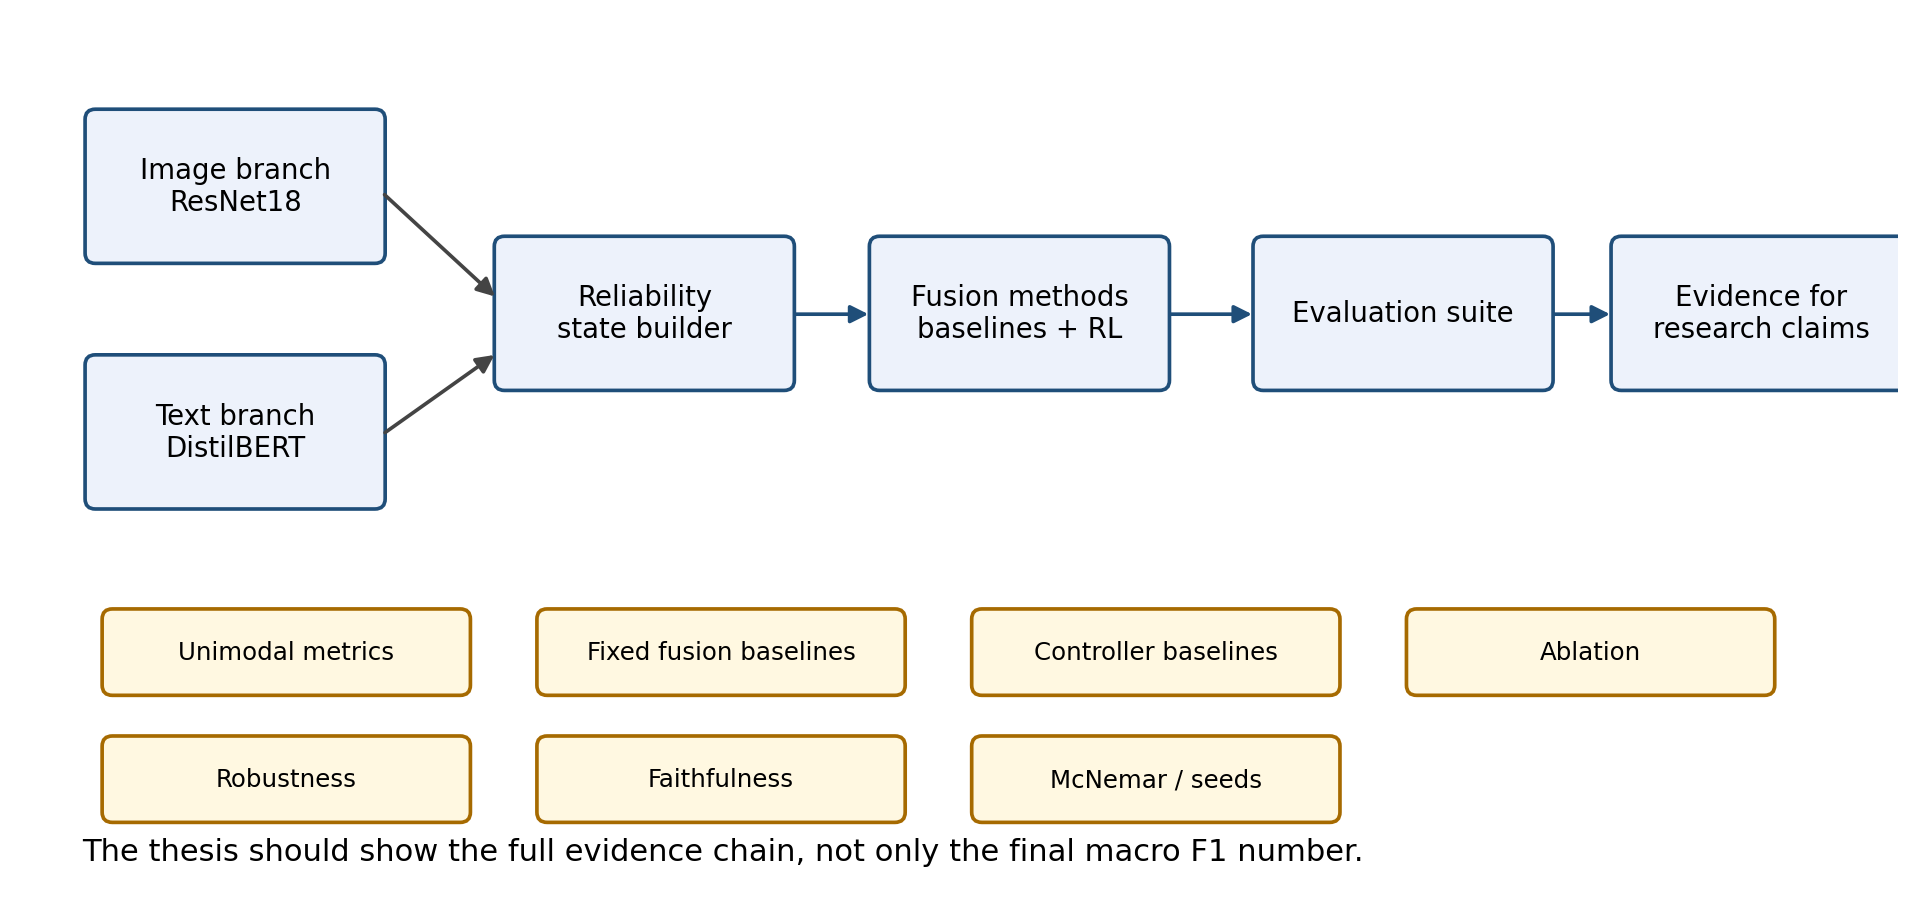
\includegraphics[width=0.92\textwidth,height=0.42\textheight,keepaspectratio]{figures/figure_7_3_final_evaluation_evidence_flow.png}
\caption{Final evaluation evidence flow across unimodal models, fusion methods, robustness, explainability, and statistical checks.}
\label{fig:evaluation_evidence_flow}
\end{figure}

\begin{table}[H]
\centering
\tiny
\caption{Dataset preparation and retention evidence for the final multimodal experiment.}
\label{tab:dataset_retention}
\begin{tabularx}{\textwidth}{YYYYY}
\toprule
stage & requested\_\allowbreak or\_\allowbreak source & available & failed\_\allowbreak or\_\allowbreak removed & evidence \\
\midrule
Full prepared metadata & 682661 & 682661 & 0 & fakeddit\_\allowbreak stats.json \\
Final requested subset & 28000 & 26471 & 1529 failed image downloads & final image download summary \\
Train split & 20000 requested & 18893 & 1107 failed & final\_\allowbreak splits\_\allowbreak available/\allowbreak train.csv \\
Validation split & 4000 requested & 3798 & 202 failed & final\_\allowbreak splits\_\allowbreak available/\allowbreak validation.csv \\
Test split & 4000 requested & 3780 & 220 failed & final\_\allowbreak splits\_\allowbreak available/\allowbreak test.csv \\
\bottomrule
\end{tabularx}
\end{table}

Macro F1 was used as the primary classification metric because it gives equal importance to both classes:

\begin{equation}
F1_{macro}=\frac{1}{C}\sum_{c=1}^{C}F1_c
\label{eq:macro_f1}
\end{equation}

Validation-threshold tuning selected the threshold that maximized validation macro F1 and then applied that threshold unchanged to the test split:

\begin{equation}
\tau^* = \arg\max_{\tau \in T} F1_{macro}^{val}(\tau)
\label{eq:threshold_tuning}
\end{equation}

\begin{figure}[H]
\centering
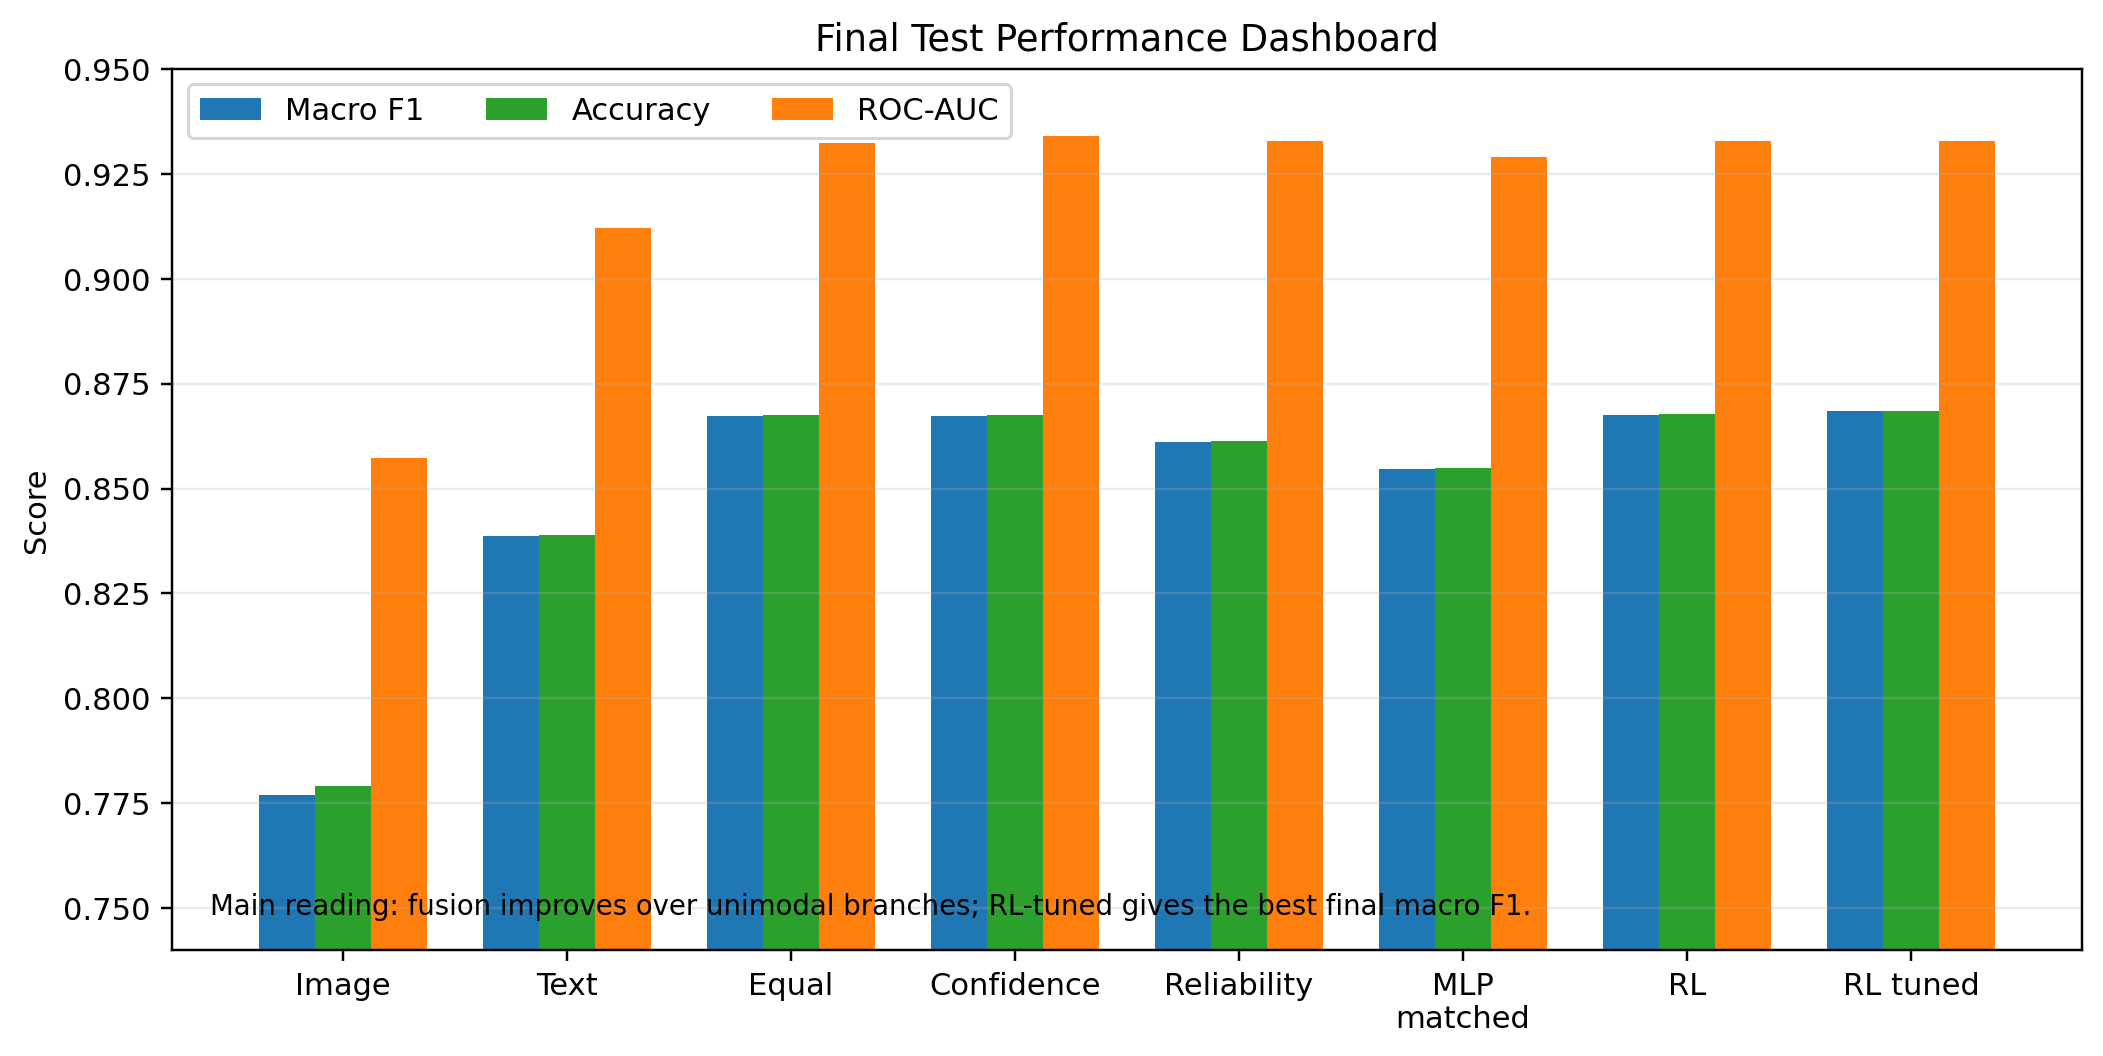
\includegraphics[width=0.92\textwidth,height=0.42\textheight,keepaspectratio]{figures/figure_7_8_final_performance_dashboard.png}
\caption{Final test performance dashboard across accuracy, macro F1, and ROC-AUC.}
\label{fig:final_performance_dashboard}
\end{figure}
\begin{figure}[H]
\centering
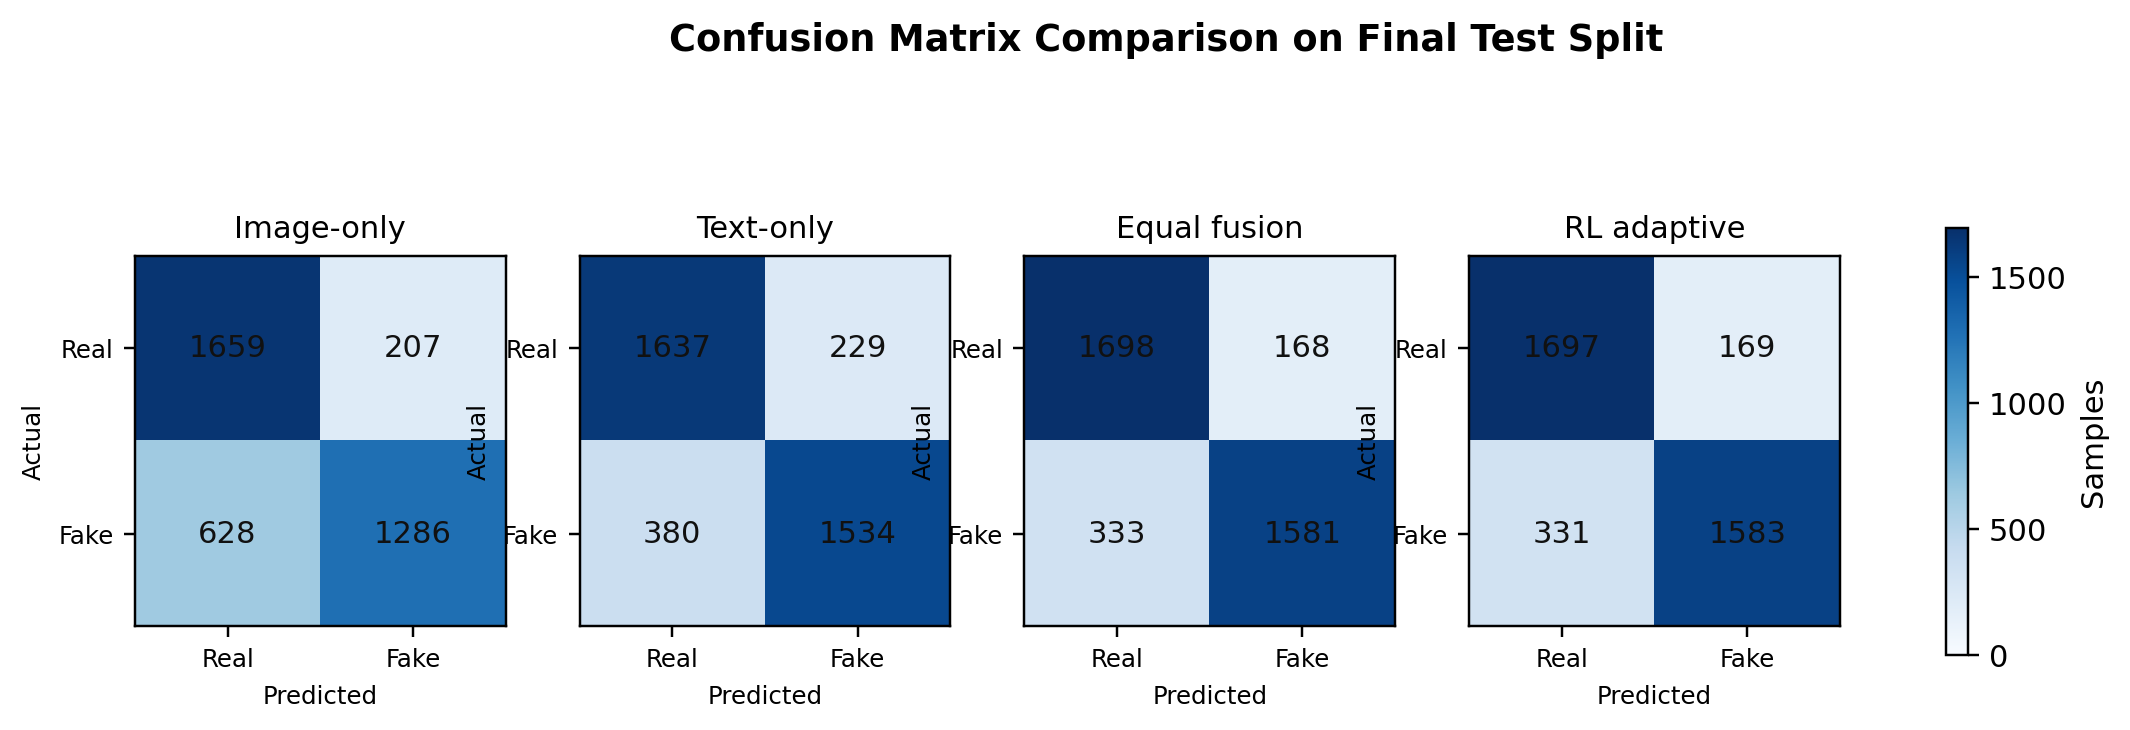
\includegraphics[width=0.92\textwidth,height=0.42\textheight,keepaspectratio]{figures/figure_7_9_confusion_matrix_panel.png}
\caption{Confusion matrix comparison for unimodal, fixed-fusion, and adaptive-fusion methods.}
\label{fig:confusion_matrix_panel}
\end{figure}
\begin{figure}[H]
\centering
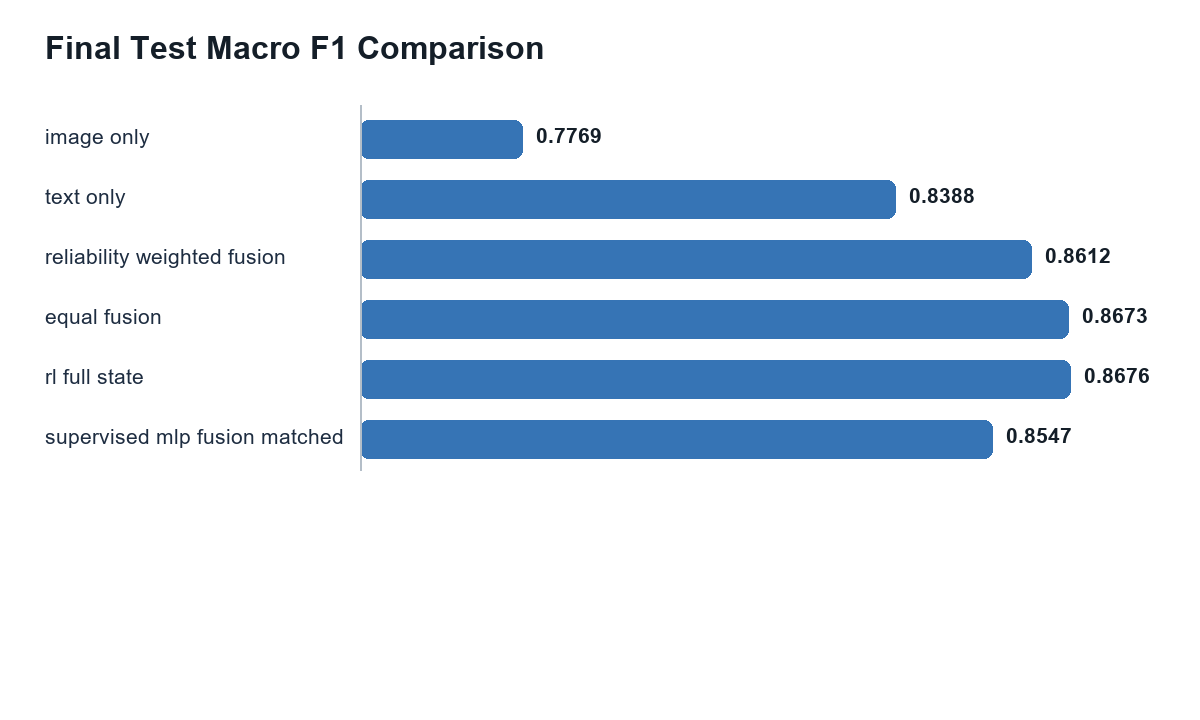
\includegraphics[width=0.92\textwidth,height=0.42\textheight,keepaspectratio]{figures/figure_7_1_method_macro_f1.png}
\caption{Final test macro F1 comparison across selected methods.}
\label{fig:method_macro_f1}
\end{figure}
\begin{table}[H]
\centering
\tiny
\caption{Final test method comparison.}
\label{tab:final_method_comparison}
\begin{tabularx}{\textwidth}{YYYYY}
\toprule
source & method & macro\_\allowbreak f1 & accuracy & roc\_\allowbreak auc \\
\midrule
rl & rl\_\allowbreak full\_\allowbreak state & 0.8676044474818365 & 0.8677248677248677 & 0.9328939130746426 \\
baseline & equal\_\allowbreak fusion & 0.8673332160630083 & 0.8674603174603175 & 0.932541682486244 \\
baseline & confidence\_\allowbreak weighted\_\allowbreak fusion & 0.8673332160630083 & 0.8674603174603175 & 0.9339962436203704 \\
ablation & rl\_\allowbreak full\_\allowbreak reliability\_\allowbreak state & 0.8673332160630083 & 0.8674603174603175 & 0.9326433197704956 \\
baseline & reliability\_\allowbreak weighted\_\allowbreak fusion & 0.8612064094284793 & 0.8613756613756614 & 0.9328661938153012 \\
ablation & rl\_\allowbreak prediction\_\allowbreak confidence & 0.8589942254358114 & 0.858994708994709 & 0.9184258596610296 \\
supervised\_\allowbreak fusion & supervised\_\allowbreak mlp\_\allowbreak fusion\_\allowbreak matched & 0.854718945966428 & 0.8547619047619047 & 0.9291012744139476 \\
ablation & rl\_\allowbreak probabilities\_\allowbreak only & 0.8523148018484805 & 0.8523809523809524 & 0.9205120839171176 \\
supervised\_\allowbreak fusion & supervised\_\allowbreak mlp\_\allowbreak fusion & 0.8499976379068706 & 0.85 & 0.9290694952630866 \\
baseline & text\_\allowbreak only & 0.838769176548389 & 0.8388888888888889 & 0.912095228815486 \\
baseline & image\_\allowbreak only & 0.7769284368078044 & 0.7791005291005291 & 0.8572159951886086 \\
\bottomrule
\end{tabularx}
\end{table}
\begin{figure}[H]
\centering
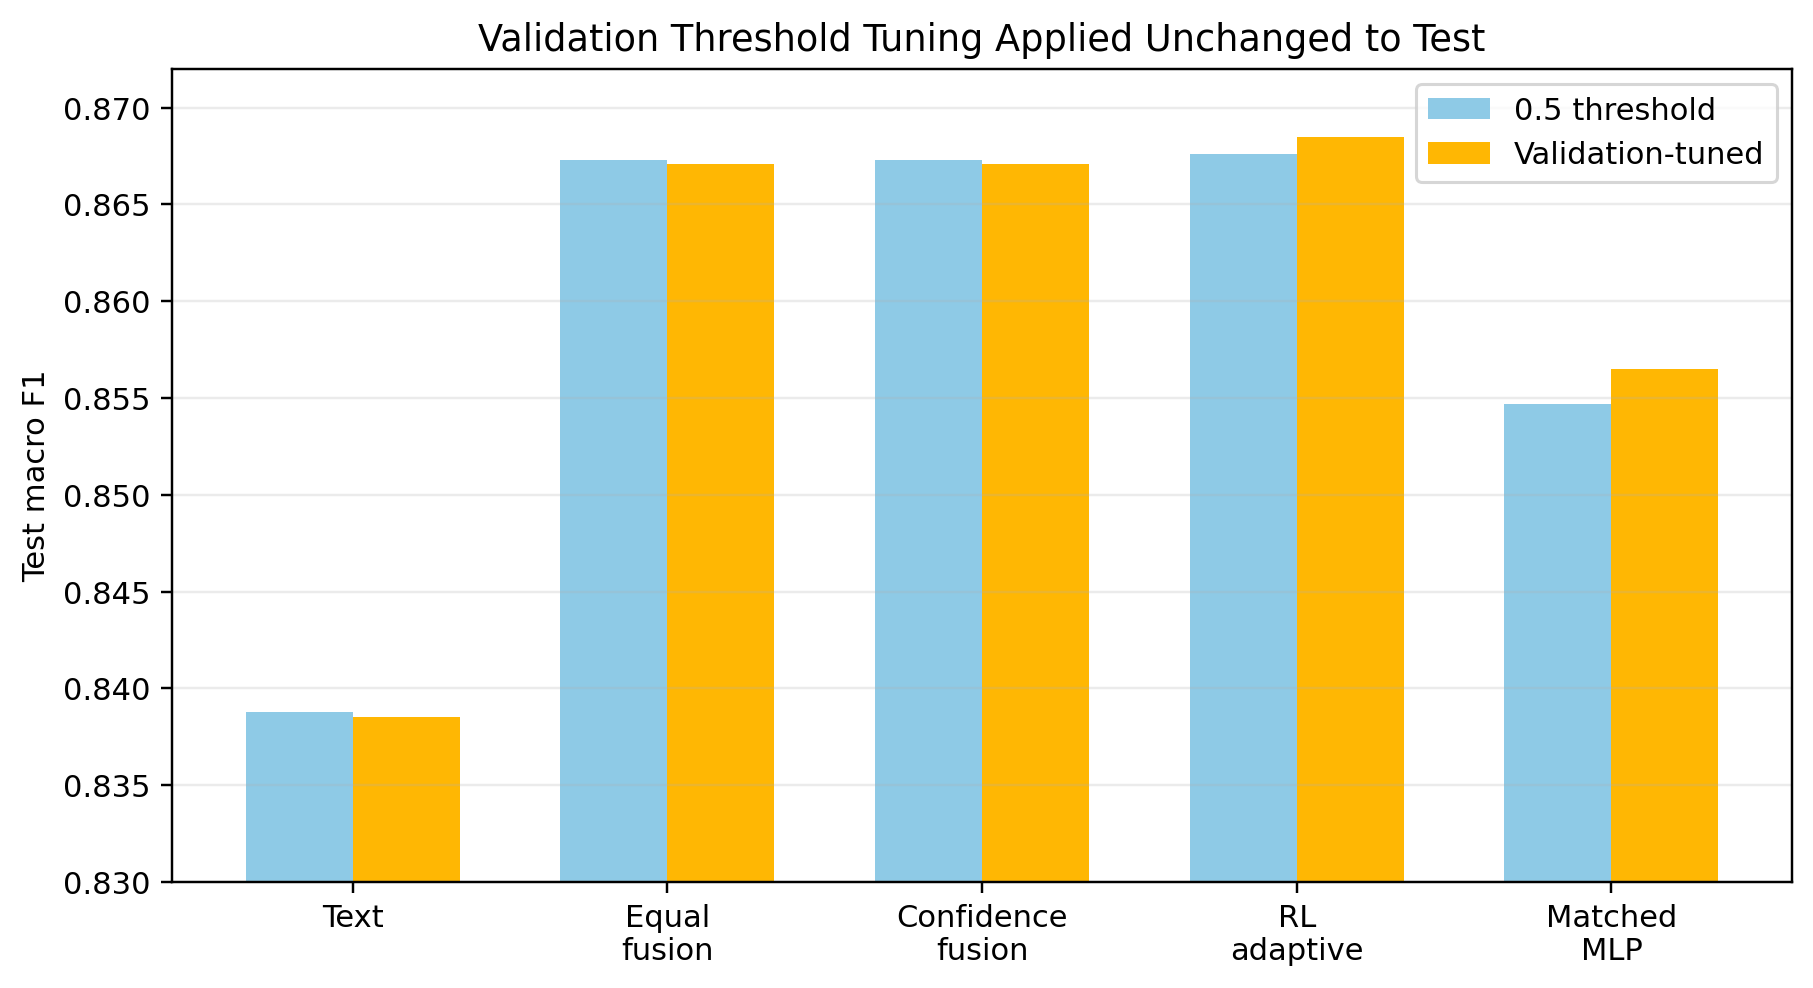
\includegraphics[width=0.92\textwidth,height=0.42\textheight,keepaspectratio]{figures/figure_7_7_threshold_tuning_comparison.png}
\caption{Comparison of default-threshold and validation-tuned threshold results.}
\label{fig:threshold_tuning_comparison}
\end{figure}

\begin{figure}[H]
\centering
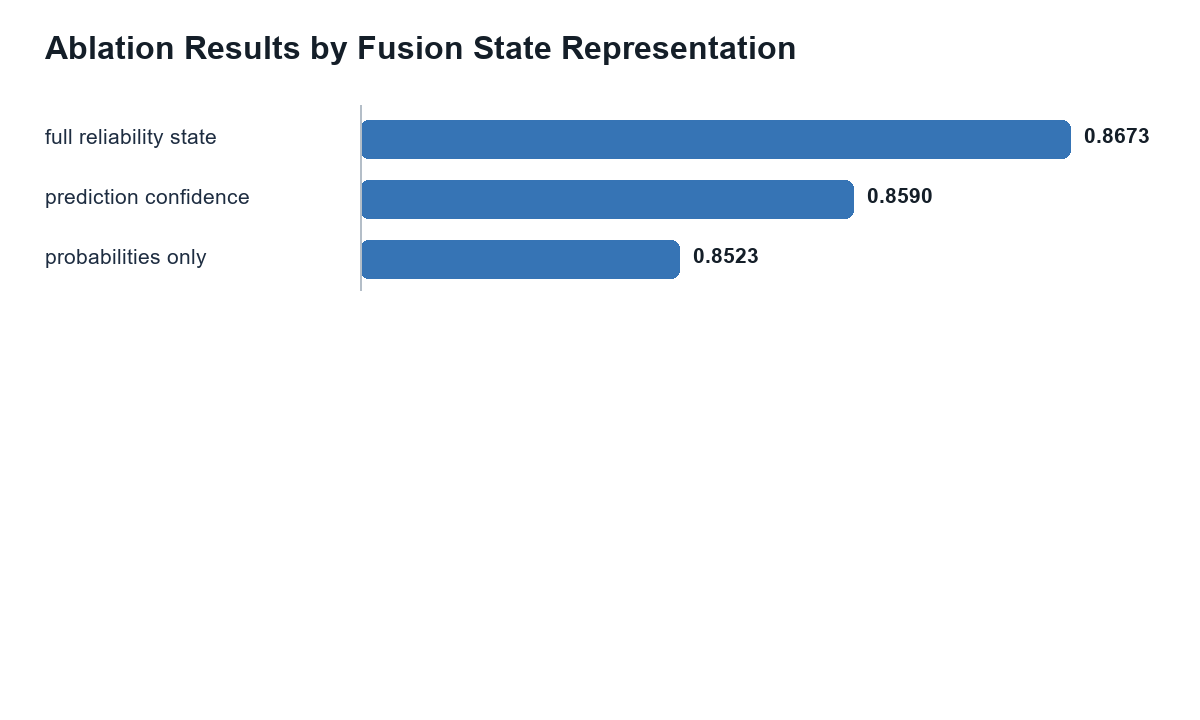
\includegraphics[width=0.92\textwidth,height=0.42\textheight,keepaspectratio]{figures/figure_7_2_ablation_macro_f1.png}
\caption{Ablation results for different RL fusion state representations.}
\label{fig:ablation_macro_f1}
\end{figure}
\begin{figure}[H]
\centering
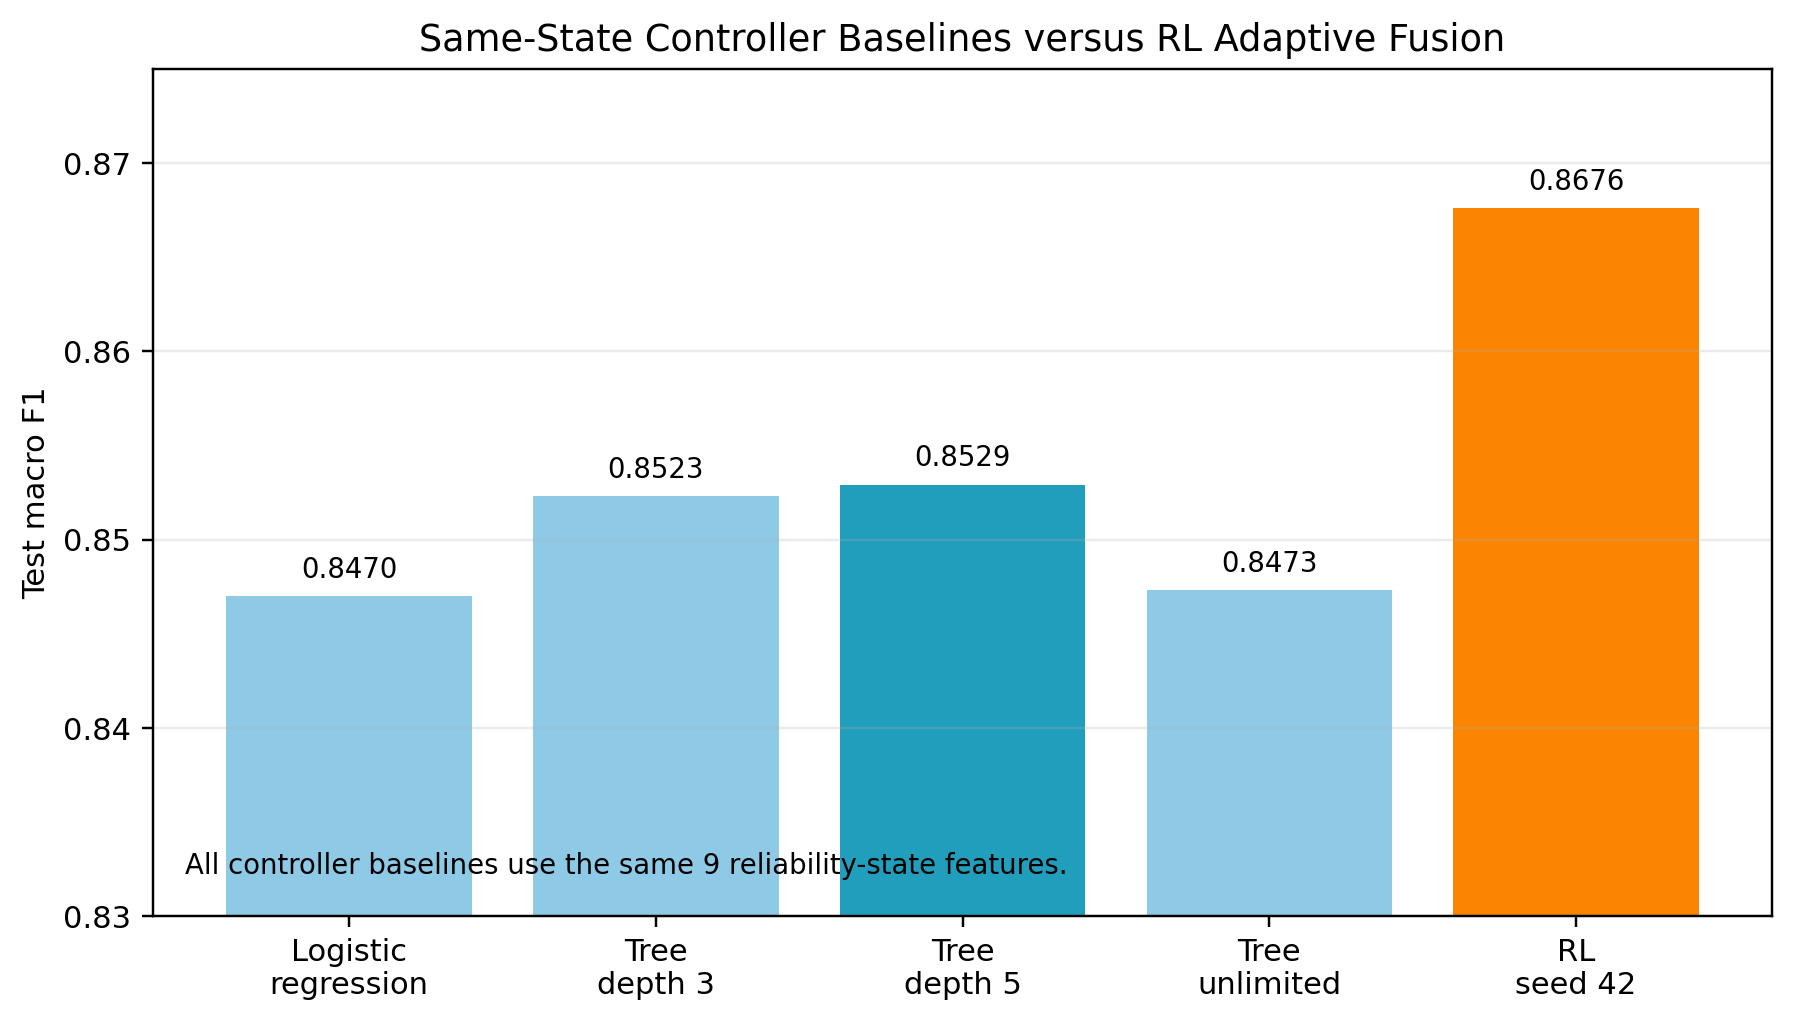
\includegraphics[width=0.92\textwidth,height=0.42\textheight,keepaspectratio]{figures/figure_7_5_controller_baseline_comparison.png}
\caption{Same-state controller baseline comparison against the RL adaptive fusion controller.}
\label{fig:controller_baseline_comparison}
\end{figure}
\begin{table}[H]
\centering
\tiny
\caption{Same-state controller baseline results.}
\label{tab:controller_baselines}
\begin{tabularx}{\textwidth}{YYYYY}
\toprule
method & state\_\allowbreak dim & validation\_\allowbreak macro\_\allowbreak f1 & test\_\allowbreak macro\_\allowbreak f1 & test\_\allowbreak accuracy \\
\midrule
state\_\allowbreak logistic\_\allowbreak regression & 9 & 0.8541 & 0.8470 & 0.8471 \\
state\_\allowbreak decision\_\allowbreak tree\_\allowbreak depth\_\allowbreak 3 & 9 & 0.8576 & 0.8523 & 0.8524 \\
state\_\allowbreak decision\_\allowbreak tree\_\allowbreak depth\_\allowbreak 5 & 9 & 0.8604 & 0.8529 & 0.8529 \\
state\_\allowbreak decision\_\allowbreak tree\_\allowbreak unlimited & 9 & 0.8541 & 0.8473 & 0.8474 \\
rl\_\allowbreak adaptive\_\allowbreak fusion\_\allowbreak seed\_\allowbreak 42 & 9 & 0.8678 & 0.8676 & 0.8677 \\
\bottomrule
\end{tabularx}
\end{table}

\begin{figure}[H]
\centering
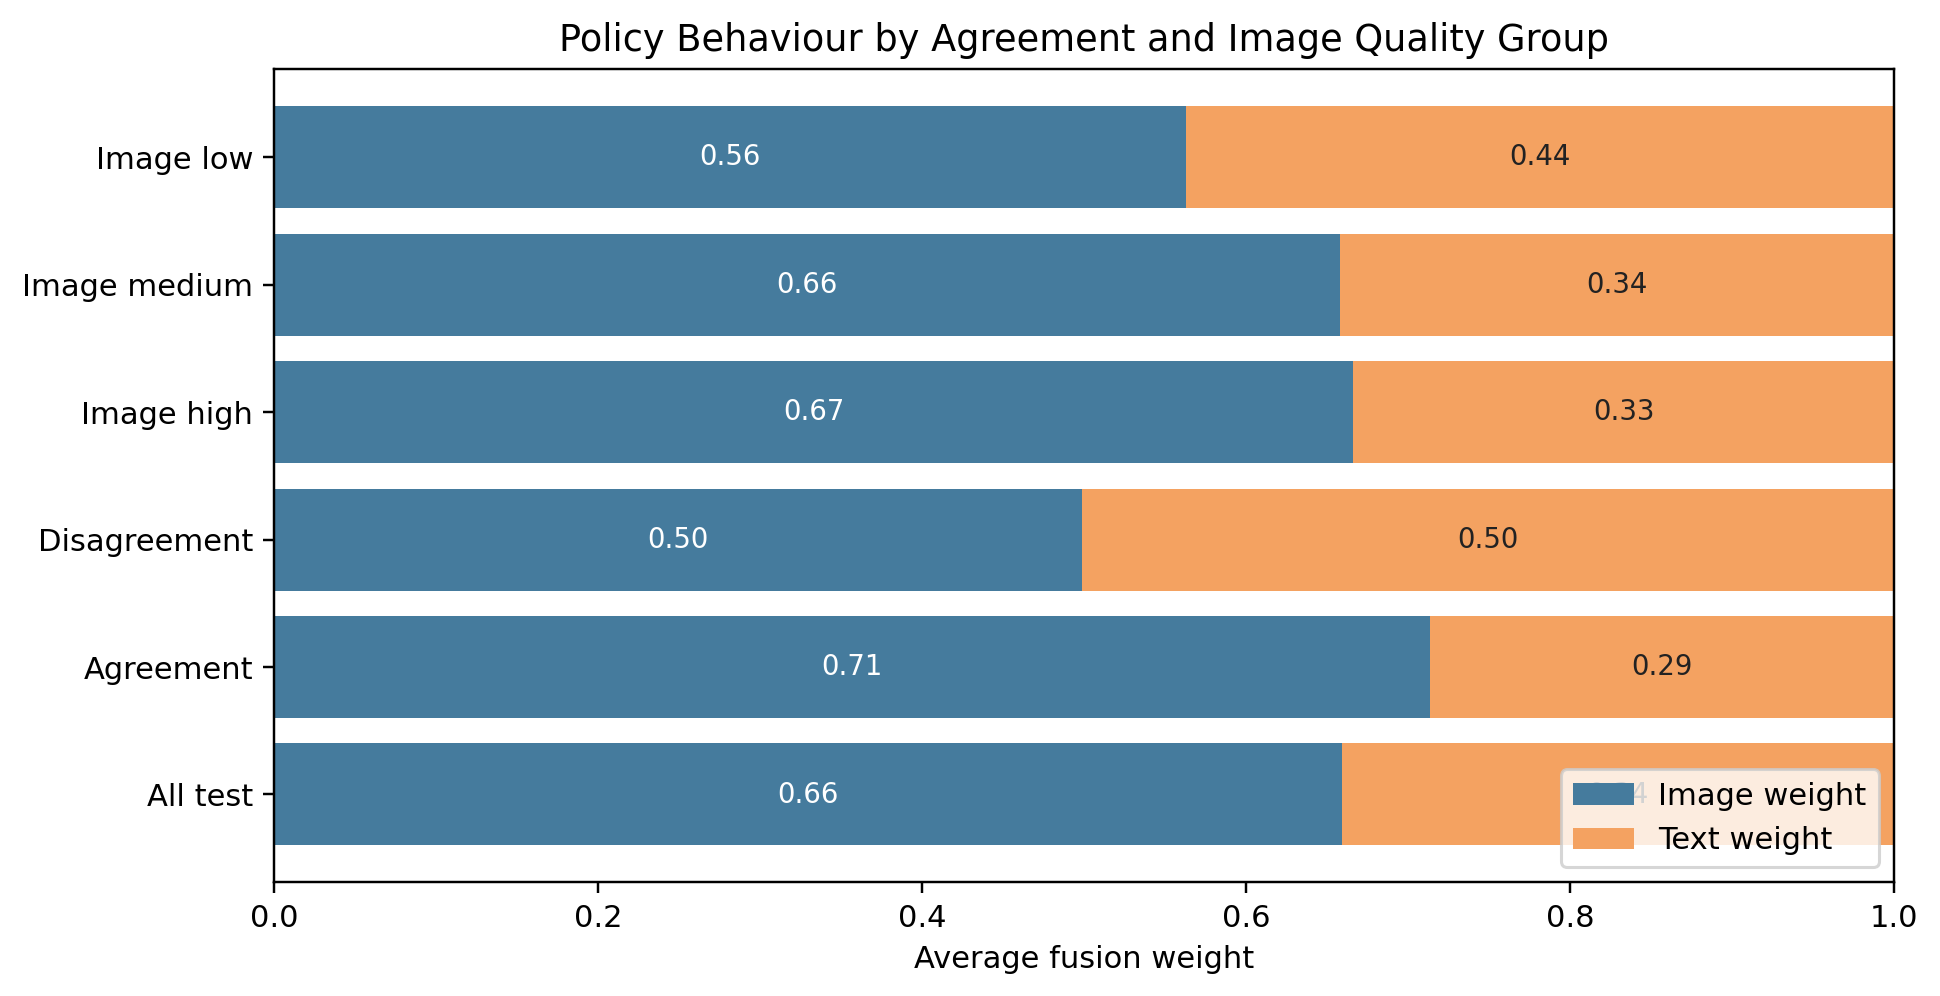
\includegraphics[width=0.92\textwidth,height=0.42\textheight,keepaspectratio]{figures/figure_7_11_modality_weight_behavior.png}
\caption{Average modality weights selected by the RL policy across agreement and image-quality groups.}
\label{fig:modality_weight_behavior}
\end{figure}
\begin{figure}[H]
\centering
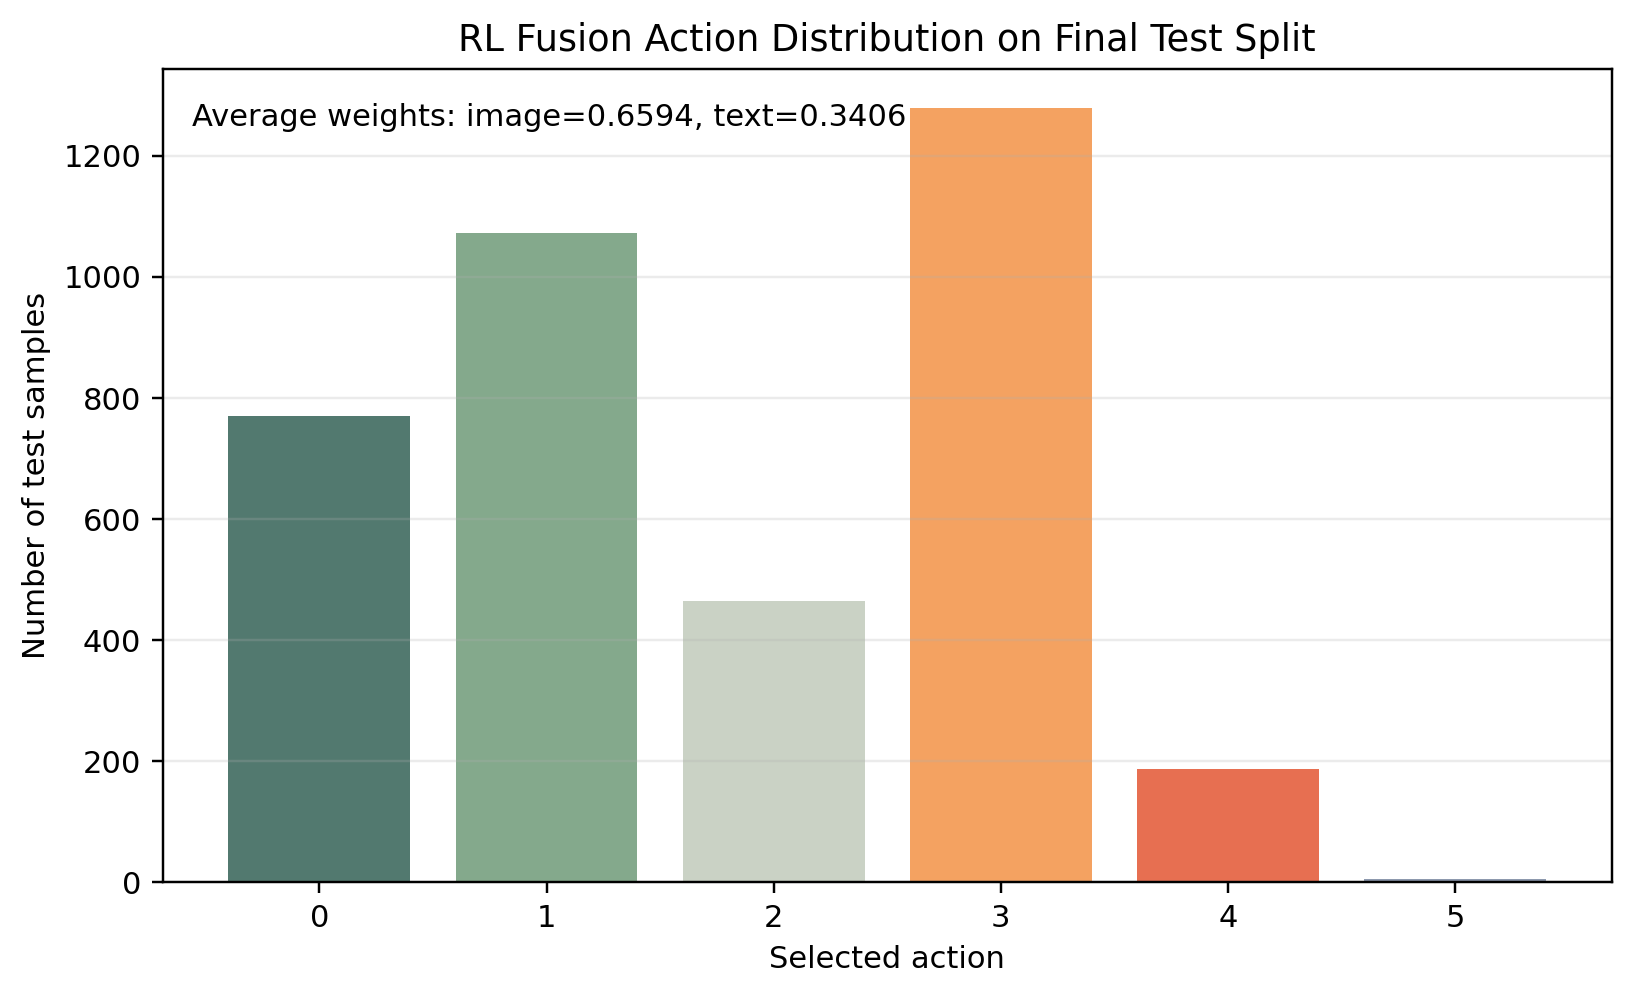
\includegraphics[width=0.92\textwidth,height=0.42\textheight,keepaspectratio]{figures/figure_7_4_policy_action_distribution.png}
\caption{Distribution of selected RL fusion actions on the final test split.}
\label{fig:policy_action_distribution}
\end{figure}

\begin{figure}[H]
\centering
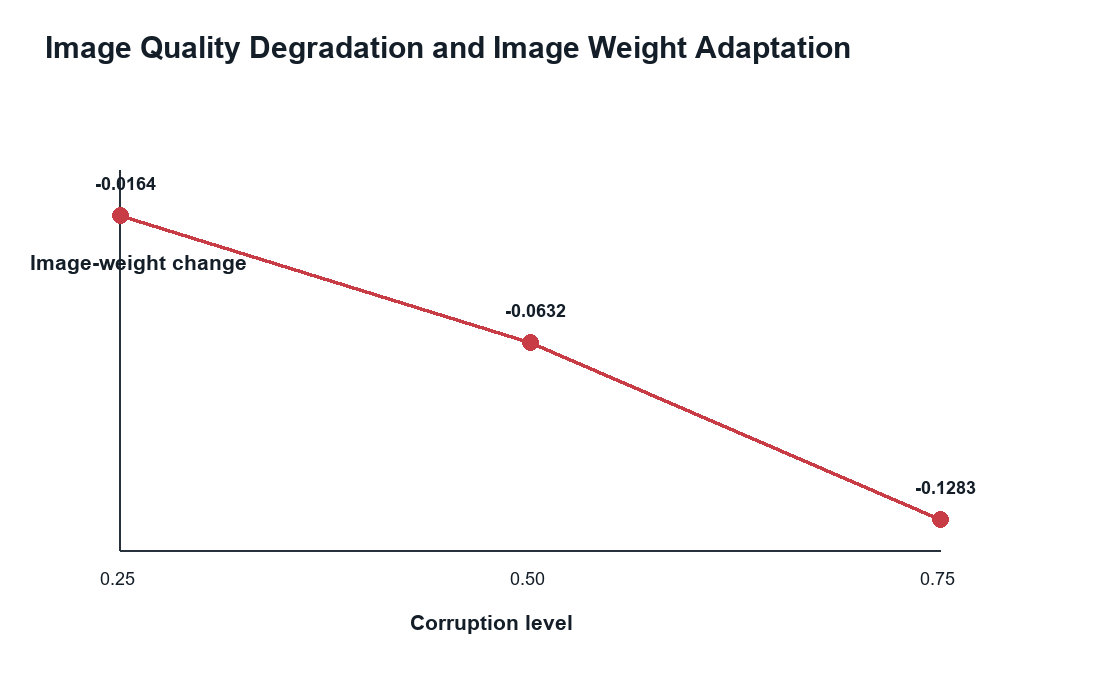
\includegraphics[width=0.92\textwidth,height=0.42\textheight,keepaspectratio]{figures/figure_7_4_robustness_image_quality.png}
\caption{Image quality degradation and image-weight adaptation.}
\label{fig:robustness_image_quality}
\end{figure}

Deletion-based faithfulness was measured using comprehensiveness, defined as the probability drop after removing evidence E:

\begin{equation}
Comp(E)=P(y_c\mid x)-P(y_c\mid x_{\setminus E})
\label{eq:faithfulness_comprehensiveness}
\end{equation}
\begin{figure}[H]
\centering
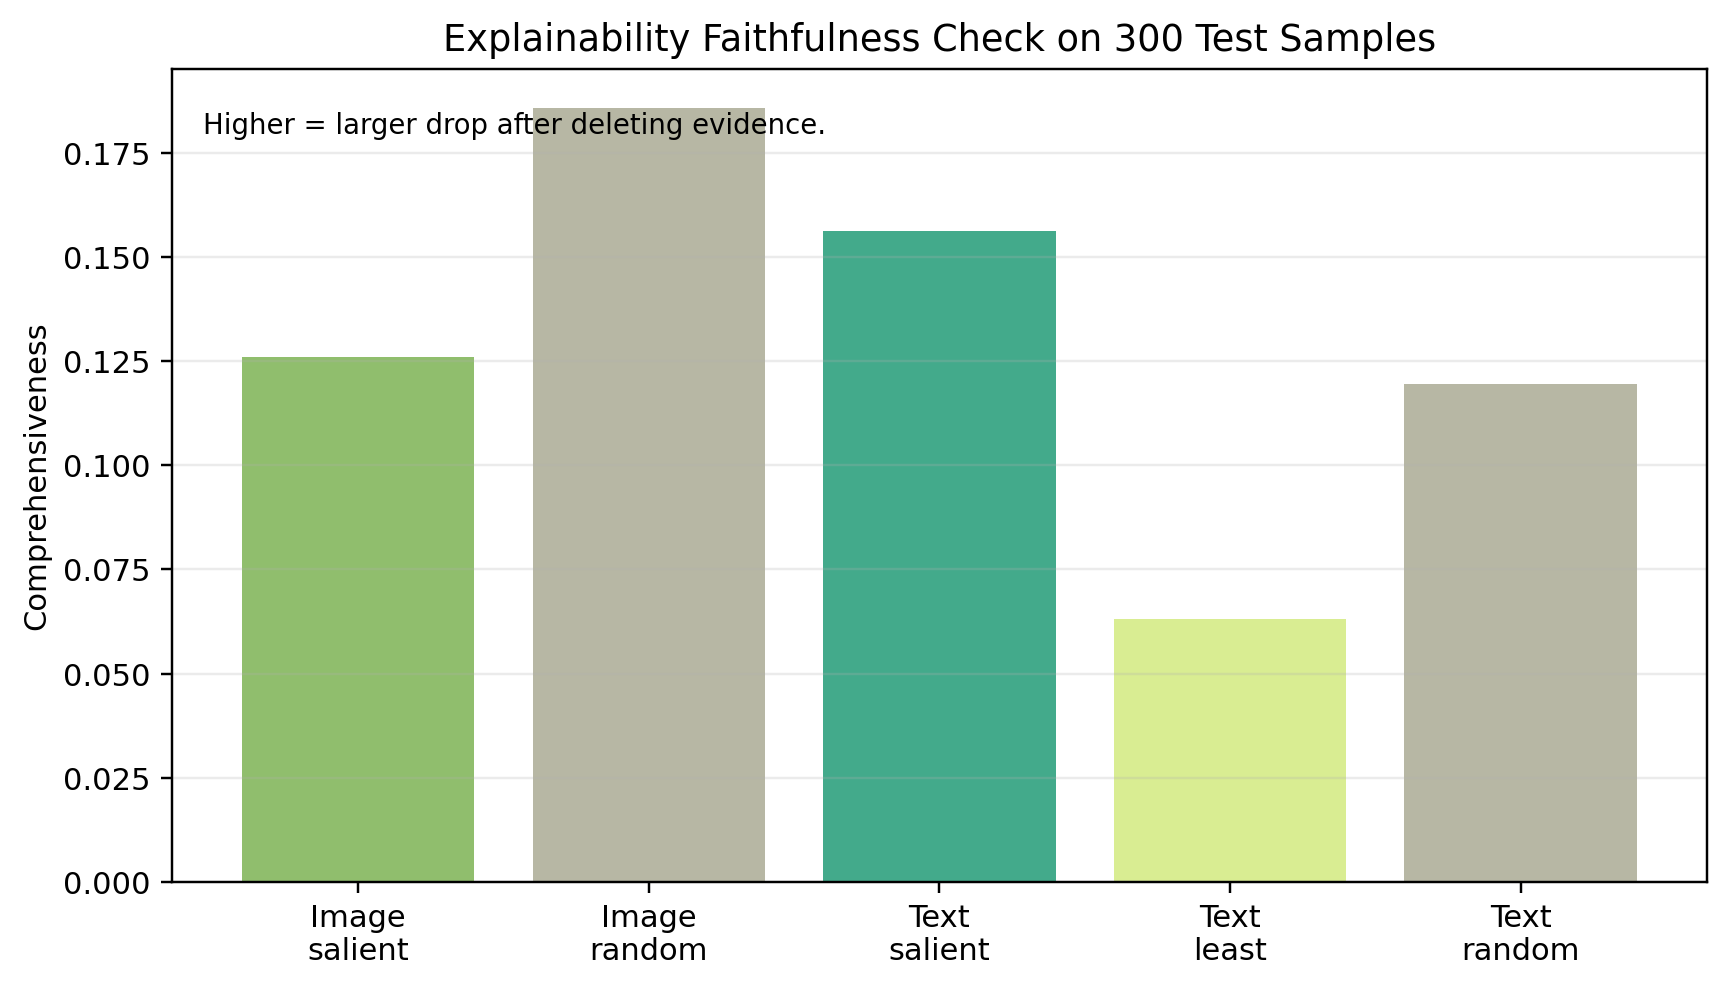
\includegraphics[width=0.92\textwidth,height=0.42\textheight,keepaspectratio]{figures/figure_7_6_explainability_faithfulness_n300.png}
\caption{Deletion-based explainability faithfulness check on 300 final test samples.}
\label{fig:faithfulness_n300}
\end{figure}
\begin{table}[H]
\centering
\tiny
\caption{Explainability faithfulness summary for image and text evidence deletion.}
\label{tab:faithfulness_n300}
\begin{tabularx}{\textwidth}{YYYYYY}
\toprule
explanation\_\allowbreak test & samples & salient & control & margin & finding \\
\midrule
image Grad-CAM deletion & 300 & 0.1260 & random 0.1858 & -0.0598 & not passed \\
text saliency vs least-salient deletion & 300 & 0.1562 & 0.0631 & 0.0931 & passed \\
text saliency vs random deletion & 300 & 0.1562 & 0.1195 & 0.0367 & passed \\
\bottomrule
\end{tabularx}
\end{table}

For paired classifier comparison, McNemar's test uses the discordant correctness counts:

\begin{equation}
b = |\{j: \hat{y}^{A}_{j}=y_j,\ \hat{y}^{B}_{j}\ne y_j\}|, \qquad c = |\{j: \hat{y}^{A}_{j}\ne y_j,\ \hat{y}^{B}_{j}=y_j\}|
\label{eq:mcnemar_counts}
\end{equation}
\begin{figure}[H]
\centering
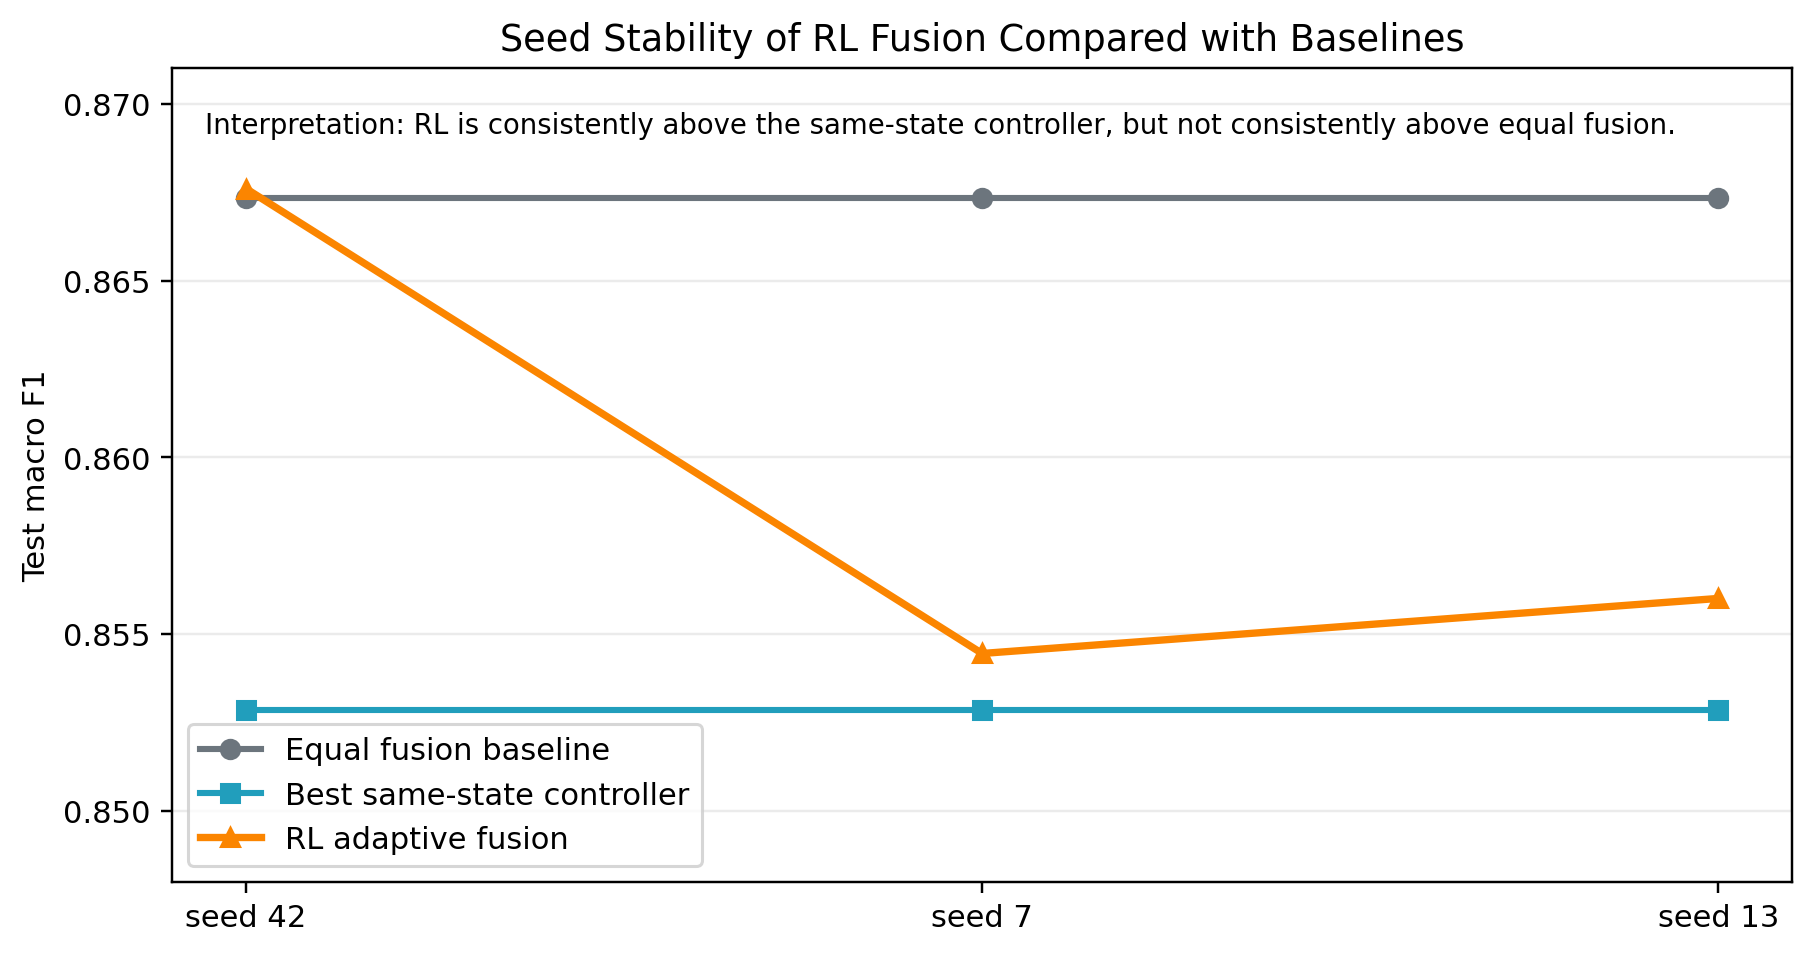
\includegraphics[width=0.92\textwidth,height=0.42\textheight,keepaspectratio]{figures/figure_7_10_seed_stability.png}
\caption{Seed-stability comparison between RL adaptive fusion, equal fusion, and the best same-state controller baseline.}
\label{fig:seed_stability}
\end{figure}

\begin{table}[H]
\centering
\tiny
\caption{External OpenFake calibration-holdout case study results.}
\label{tab:external_openfake_calibration}
\begin{tabularx}{\textwidth}{YYYYY}
\toprule
Method & Selected threshold & Holdout macro F1 & Holdout accuracy & Holdout ROC-AUC \\
\midrule
text\_\allowbreak only & 0.991 & 0.858926 & 0.859127 & 0.859127 \\
rl\_\allowbreak adaptive\_\allowbreak fusion & 0.889 & 0.489392 & 0.490410 & 0.474842 \\
equal\_\allowbreak fusion & 0.894 & 0.484248 & 0.485450 & 0.478006 \\
image\_\allowbreak only & 0.788 & 0.480838 & 0.481812 & 0.468784 \\
\bottomrule
\end{tabularx}
\end{table}

\begin{table}[H]
\centering
\tiny
\caption{Research-question and examiner-question evidence mapping.}
\label{tab:research_question_evidence}
\begin{tabularx}{\textwidth}{YYY}
\toprule
examiner\_\allowbreak question & test\_\allowbreak or\_\allowbreak evidence & main\_\allowbreak finding \\
\midrule
Novelty and architecture difference & adaptive fusion architecture; same-state controller baselines & sample-level RL action and weights provide inspectable fusion \\
Baseline comparison & image/\allowbreak text/\allowbreak equal/\allowbreak confidence/\allowbreak reliability/\allowbreak MLP/\allowbreak RL comparisons & RL competitive; threshold-tuned RL macro F1 0.8685 \\
Why reliability features & state ablation & full reliability state outperformed probability-only and confidence states \\
Dataset filtering & download and validation statistics & 26,471 final multimodal rows retained; failures recorded \\
Generalizability & threats-to-validity analysis & claims restricted to Fakeddit; cross-dataset work remains future work \\
Explainability & Grad-CAM, token saliency, fusion weights, N=300 faithfulness & text saliency positive; image faithfulness remains limited \\
\bottomrule
\end{tabularx}
\end{table}

\clearpage
